\documentclass[polish,a4paper]{article}
\usepackage[utf8]{inputenc}
\usepackage[T1]{fontenc}
%%\usepackage{polski}
\usepackage{amsmath}
\usepackage{amssymb,amsfonts,amsthm}
\usepackage{babel}
\usepackage{hyperref}
\usepackage{xcolor}
\usepackage{graphicx}
\usepackage{caption}
\usepackage{subcaption}
\usepackage{listings}
\usepackage{anysize}
%%\usepackage{tabto}

\graphicspath{ {img/} }
\marginsize{2.5cm}{2.5cm}{0cm}{3cm}

\definecolor{codegreen}{rgb}{0,0.6,0}
\definecolor{codegray}{rgb}{0.5,0.5,0.5}
\definecolor{codepurple}{rgb}{0.58,0,0.82}
\definecolor{backcolour}{rgb}{0.95,0.95,0.92}

\lstdefinestyle{mystyle}{
	backgroundcolor=\color{backcolour},
	commentstyle=\color{codegreen},
	keywordstyle=\color{magenta},
	numberstyle=\tiny\color{codegray},
	stringstyle=\color{codepurple},
	basicstyle=\ttfamily\footnotesize,
	breakatwhitespace=false,
	breaklines=true,
	captionpos=b,
	keepspaces=true,
	numbers=left,
	numbersep=5pt,
	showspaces=false,
	showstringspaces=false,
	showtabs=false,
	tabsize=2
}

\lstset{style=mystyle}

\begin{document}
	\begin{center}
		\begin{tabular}{ p{0.32\textwidth} p{0.15\textwidth} p{0.15\textwidth} p{0.12\textwidth} p{0.12\textwidth} }

			&   &   &   &  \\
			\hline
			\multicolumn{5}{|c|}{}\\[-1ex]
			\multicolumn{5}{|c|}{{\LARGE \textbf{Laboratorium z przedmiotu Systemy wbudowane (SW)}}}\\
			\multicolumn{5}{|c|}{}\\[-1ex]
			\hline
			\hline

			\multicolumn{5}{|c|}{}\\[-1ex]
			\multicolumn{5}{|c|}{{\LARGE Zadanie nr 5}}\\
			\multicolumn{5}{|c|}{}\\[-1ex]
			\hline
			\hline

			\multicolumn{5}{|c|}{}\\[-1ex]
			\multicolumn{5}{|c|}{{\textbf{Temat zajęć:} BeagleBone Black – baza danych}}\\
			\multicolumn{5}{|c|}{}\\[-1ex]
			\hline
			\hline

			\multicolumn{1}{|l|}{Prowadzący} &
			\multicolumn{2}{|l|}{Autorzy} &
			\multicolumn{2}{|l|}{Grupa dziekańska:} \\
			\multicolumn{1}{|c|}{mgr inż. Ariel Antonowicz} &
			\multicolumn{2}{|c|}{148088 i 148121} &
			\multicolumn{2}{|c|}{I1.2} \\
			\hline
			\hline
		\end{tabular}
	\end{center}
    \[\,\]
	\section{Zapis pomiaru do bazy danych - DHT11}
	\begin{figure}[h!]
		\begin{center}
			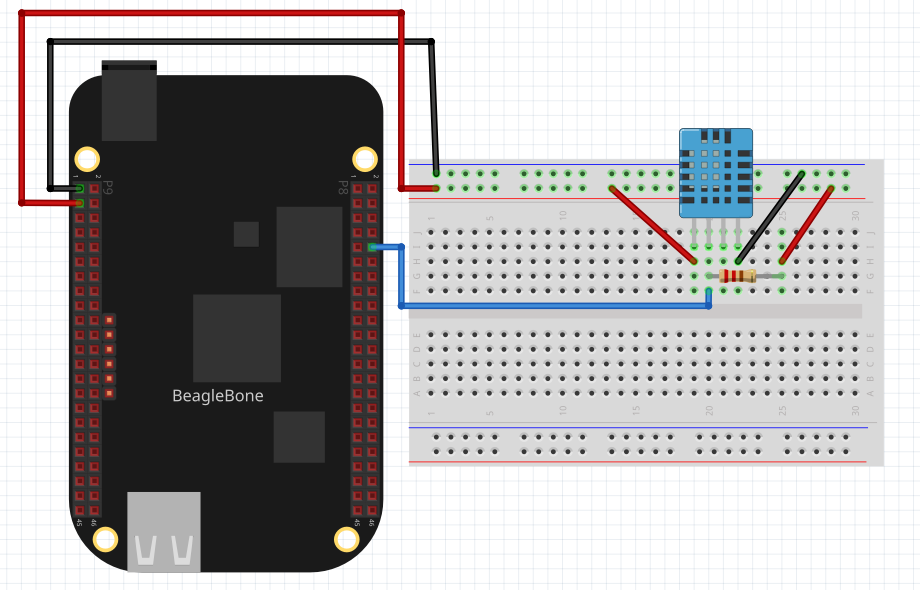
\includegraphics[scale=0.7]{dht11.png}
			\caption*{Schemat podłączenia czujnika do BeagleBone'a}
		\end{center}
	\end{figure}
 \newpage
	\begin{figure}[h!]
		\begin{lstlisting}[language=python,basicstyle=\scriptsize]
#!/usr/bin/python
import Adafruit_DHT
import datetime
import sqlite3
from sqlite3 import Error


def create_connection(db):
    con = None
    try:
        con = sqlite3.connect(db)
    except Error as e:
        print(e)
    return con


def create_table(con, create_sql):
    try:
        c = con.cursor()
        c.execute(create_sql)
        c.close()
    except Error as e:
        print(e)


def insert2db(con, val):
    sql_insert = "INSERT INTO measurements(temp, hum, date) VALUES(?,?,?)"
    cur = con.cursor()
    cur.execute(sql_insert, val)
    con.commit()
    cur.close()


def return_table(con):
    cur = con.cursor()
    cur.execute("SELECT * from measurements")
    rows = cur.fetchall()
    for row in rows:
        print(row)
    cur.close()


conn = create_connection('pysqlite.db')
sql_create = "CREATE TABLE IF NOT EXISTS measurements (id INTEGER PRIMARY KEY AUTOINCREMENT, temp REAL, hum REAL, date TIMESTAMP);"
create_table(conn, sql_create)

sensor = Adafruit_DHT.DHT11
pin = 'P8_10'
temp = []
hum = []

read = True # zmienic na false zeby wyswietlic dane z tabeli

if read:
    while True:
        humidity, temperature = Adafruit_DHT.read_retry(sensor, pin)
        if humidity is not None and temperature is not None:
            temp.append(temperature)
            hum.append(humidity)

            if len(temp) == 18:
                temp.remove(max(temp)); temp.remove(min(temp))
                t = sum(temp)/len(temp)

                hum.remove(max(hum)); hum.remove(min(hum))
                h = sum(hum)/len(hum)

                d = datetime.datetime.now()
                values = (t, h, d)
                insert2db(conn, values)

                temp.clear()
                hum.clear()
        else:
            print('Failed to get reading. Try again!')
else:
    return_table(conn)
		\end{lstlisting}
		\caption*{Kod odpowiedzialny za połączenie i komunikacje z bazą danych oraz odczytywanie danych z sensora}
	\end{figure}


	\newpage

	\section*{Źródła}
	\begin{enumerate}
		\item \href{https://forum.fritzing.org/}{Fritzing}
		\item Materiały podane przez prowadzącego na platformie ekursy.
		\item \href{https://github.com/adafruit/Fritzing-Library/blob/master/parts/BeagleBone%20Black.fzpz}{BeagleBone Black.fzpz}
        \item \href{https://github.com/adafruit/Fritzing-Library/blob/master/parts/DHT11%20Humitidy%20and%20Temperature%20Sensor.fzpz}{DHT11}
	\end{enumerate}
	\begingroup
	\hypersetup{hidelinks}
	\tableofcontents
	\endgroup
\end{document}
